\documentclass[border=10pt,preview]{standalone}

% Plots
\usepackage{graphicx}
\usepackage{tikz,pgf,pgfplots,pgfplotstable}
\usetikzlibrary{matrix}
\usepgfplotslibrary{groupplots}
\pgfplotsset{compat=1.9}
\usepackage{csvsimple,longtable,booktabs}
\usepackage{pdfpages}
% Inkscape plots
\graphicspath{{Figures/}}

\begin{document}

\begin{figure}[!htb]
\centering
\begin{tiny} % For text embedded in figure
\def\svgwidth{\linewidth}
\input{Figures/pod2_schematic.pdf_tex}
\end{tiny}
\caption{Schematic of the data center module POD 2.}
\label{fig:floor_plan}
\end{figure}

\begin{table}[h]
\caption{The RMS of the difference between simulated and experimental temperatures in C at different positions on the server racks.}
\begin{center}
	\begin{tabular}{|l|m{1.4cm}|m{1.4cm}|m{1.4cm}|m{1.4cm}|m{1.4cm}|m{1.4cm}|}%
	\hline
	\bfseries Rack & \bfseries Front Bottom & \bfseries Front Mid & \bfseries Front Top & \bfseries Back Bottom & \bfseries Back Mid & \bfseries Back Top
	\csvreader[head to column names]{Plots/P02RX_T_rms.csv}{}% use head of csv as column names
	{\\\hline\rack&\Tinb&\Tinm&\Tint&\Toutb&\Toutm&\Toutt}% specify your coloumns here
	\\\hline
	\end{tabular}
\end{center}
\label{tab:rms_rack_temps}
\end{table}

% P02HDZ01
\begin{figure}[!htb]
\centering
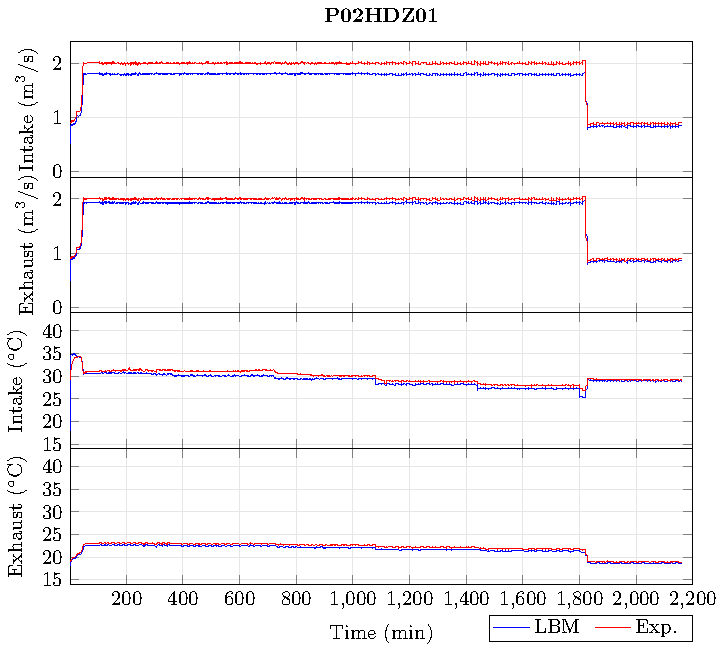
\includegraphics[width=\linewidth]{Plots/P02HDZ01_T.pdf}
\caption{Comparison of simulated and experimental temperatures for CRAC unit P02HDZ01.}
\label{fig:P02HDZ01_plot}
\end{figure}

\clearpage

% P02HDZ02
\begin{figure}[!htb]
\centering
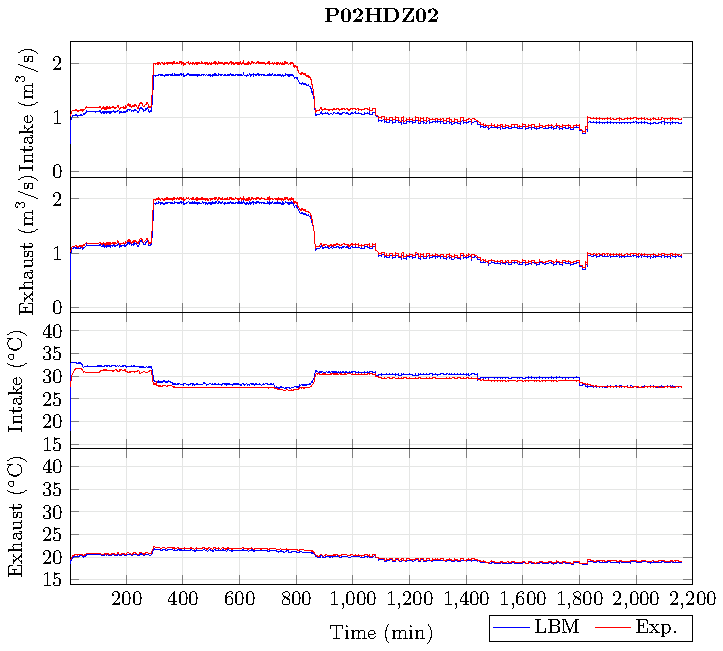
\includegraphics[width=\linewidth]{Plots/P02HDZ02_T.pdf}
\caption{Comparison of simulated and experimental temperatures for CRAC unit P02HDZ02.}
\label{fig:P02HDZ02_plot}
\end{figure}

\clearpage

% P02HDZ03
\begin{figure}[!htb]
\centering
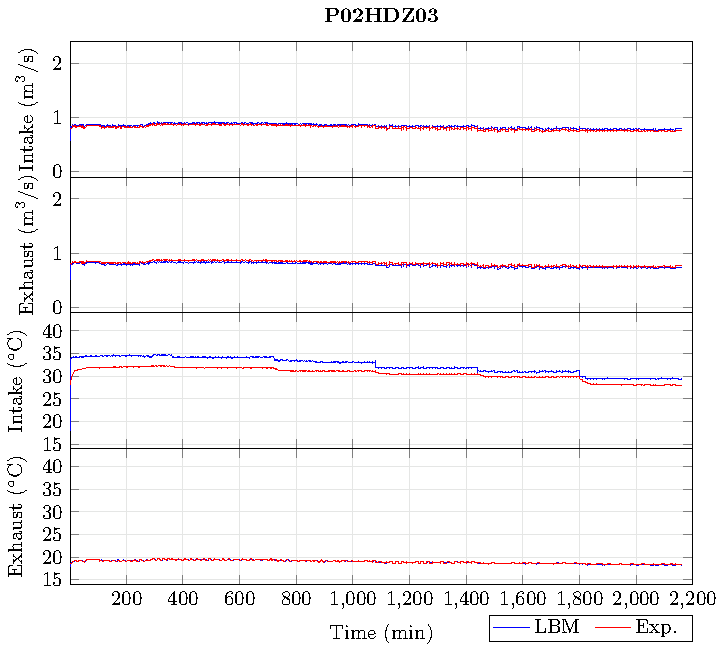
\includegraphics[width=\linewidth]{Plots/P02HDZ03_T.pdf}
\caption{Comparison of simulated and experimental temperatures for CRAC unit P02HDZ03.}
\label{fig:P02HDZ03_plot}
\end{figure}

\clearpage

% P02HDZ04
\begin{figure}[!htb]
\centering
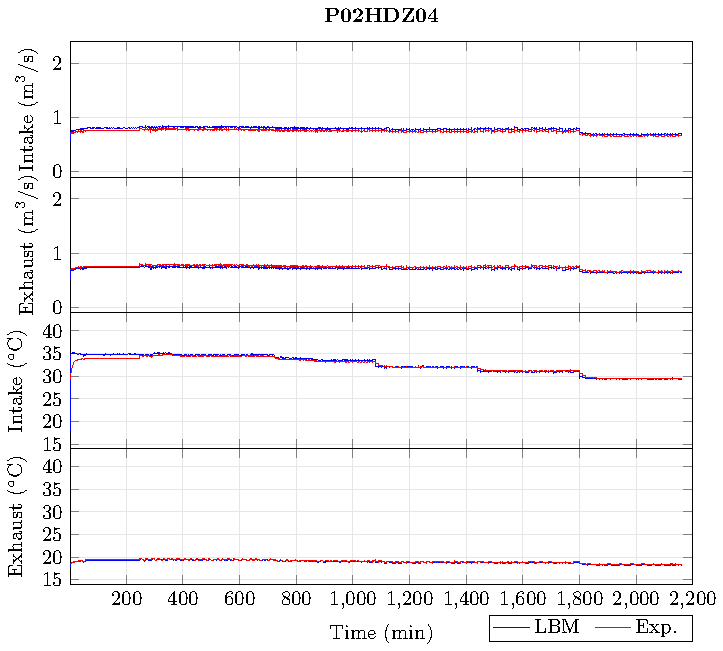
\includegraphics[width=\linewidth]{Plots/P02HDZ04_T.pdf}
\caption{Comparison of simulated and experimental temperatures for CRAC unit P02HDZ04.}
\label{fig:P02HDZ04_plot}
\end{figure}


\clearpage

% P02R01
\begin{figure}[!htb]
\centering
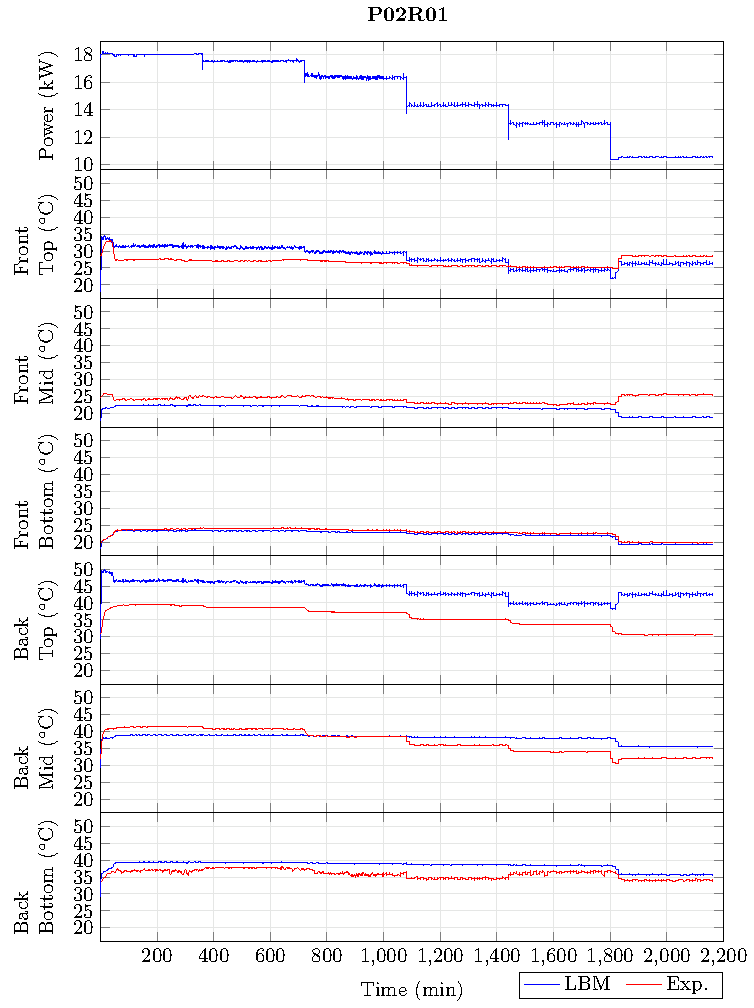
\includegraphics[width=\linewidth]{Plots/P02R01_T.pdf}
\caption{Comparison of simulated and experimental temperatures for server P02R01.}
\label{fig:P02R01_plot}
\end{figure}

\clearpage

% P02R02
\begin{figure}[!htb]
\centering
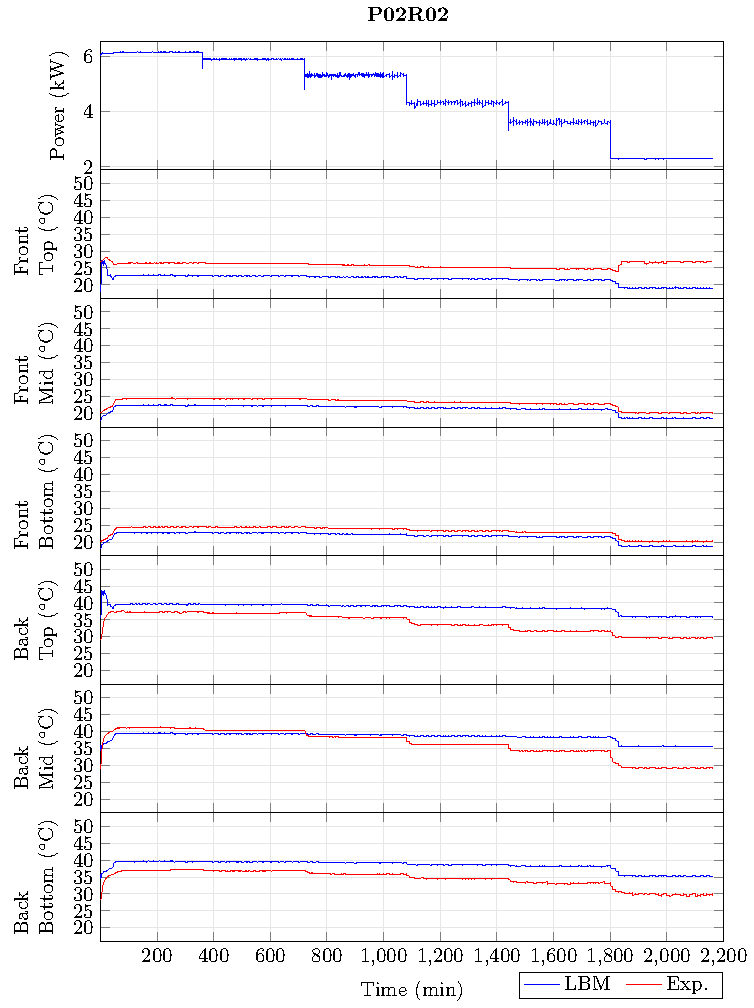
\includegraphics[width=\linewidth]{Plots/P02R02_T.pdf}
\caption{Comparison of simulated and experimental temperatures for server P02R02.}
\label{fig:P02R02_plot}
\end{figure}

\clearpage

% P02R03
\begin{figure}[!htb]
\centering
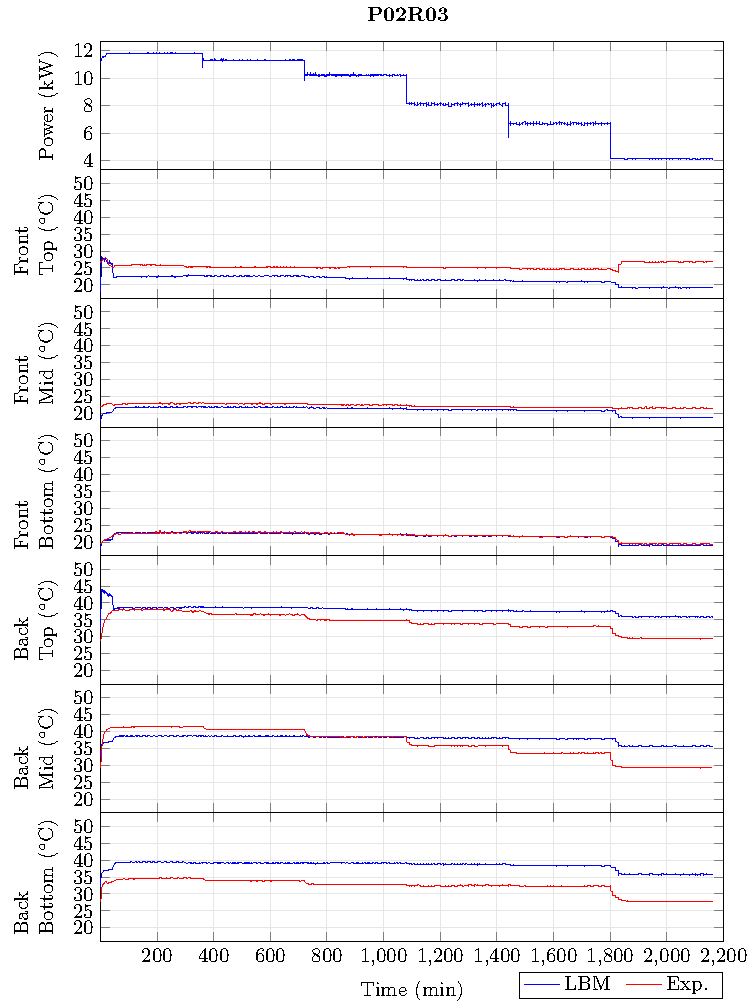
\includegraphics[width=\linewidth]{Plots/P02R03_T.pdf}
\caption{Comparison of simulated and experimental temperatures for server P02R03.}
\label{fig:P02R03_plot}
\end{figure}

\clearpage

% P02R04
\begin{figure}[!htb]
\centering
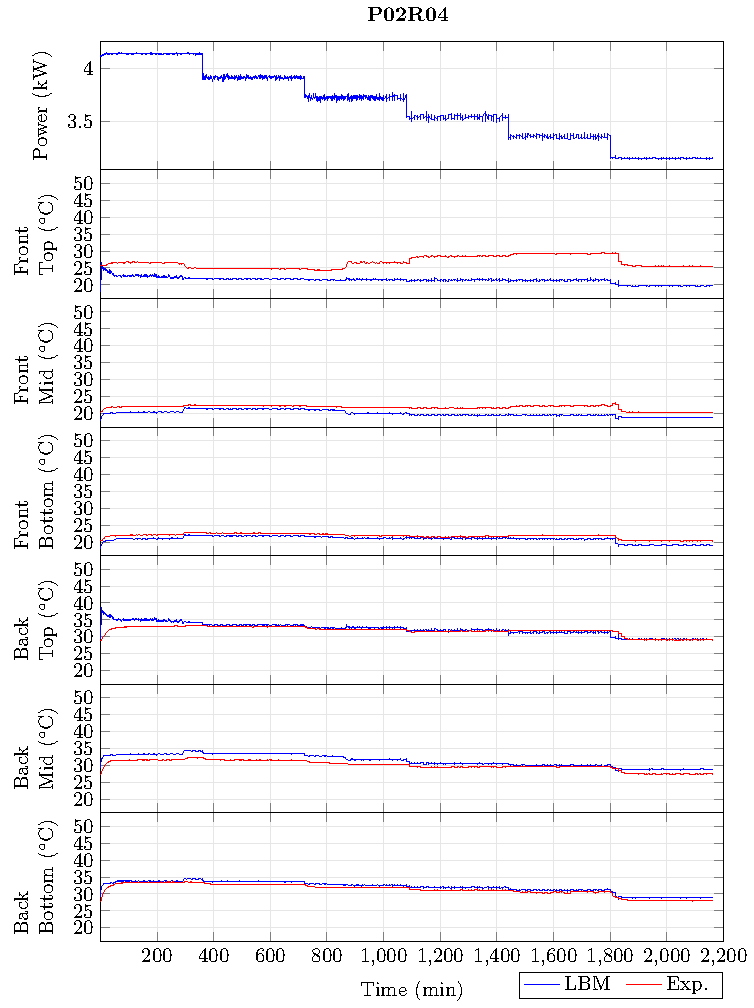
\includegraphics[width=\linewidth]{Plots/P02R04_T.pdf}
\caption{Comparison of simulated and experimental temperatures for server P02R04.}
\label{fig:P02R04_plot}
\end{figure}

\clearpage

% P02R05
\begin{figure}[!htb]
\centering
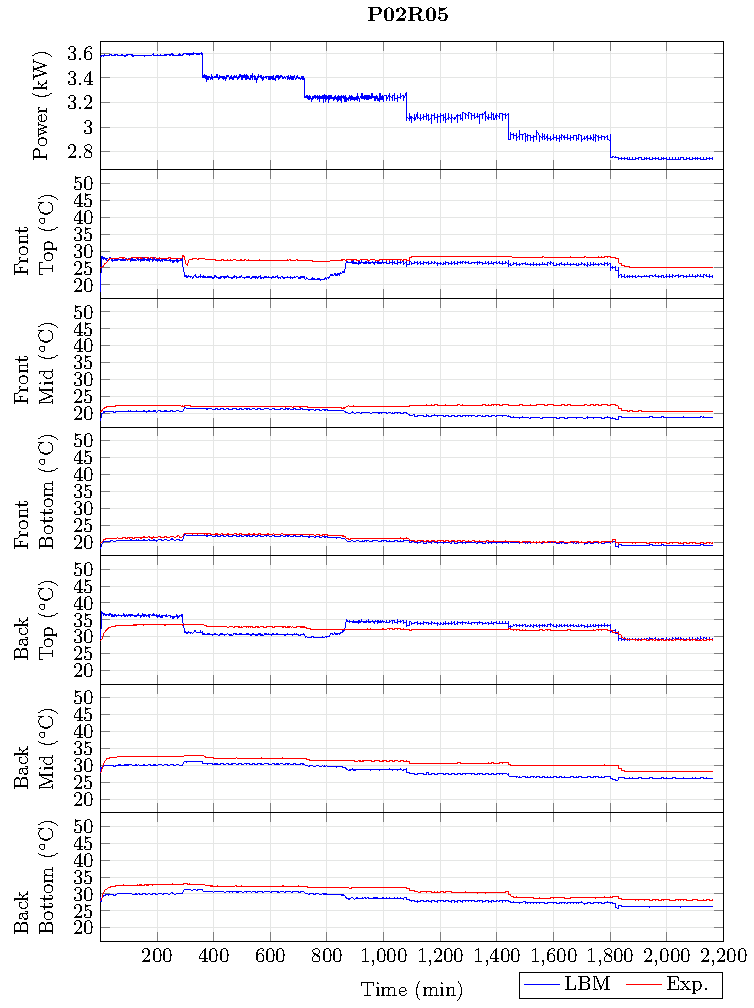
\includegraphics[width=\linewidth]{Plots/P02R05_T.pdf}
\caption{Comparison of simulated and experimental temperatures for server P02R05.}
\label{fig:P02R05_plot}
\end{figure}

\clearpage

% P02R06
\begin{figure}[!htb]
\centering
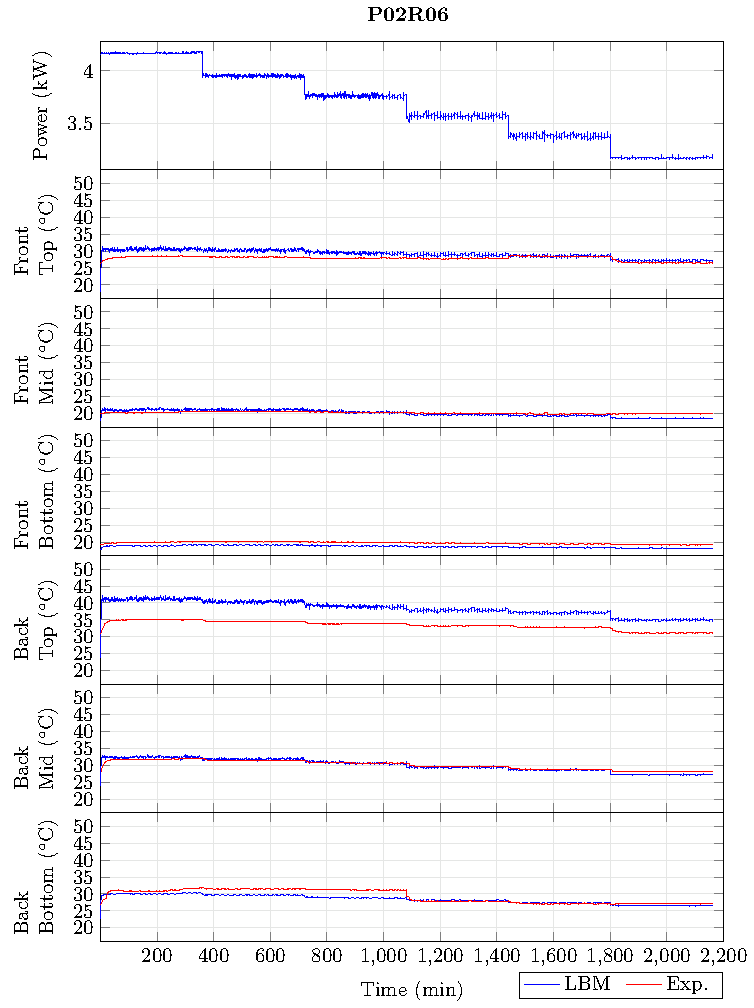
\includegraphics[width=\linewidth]{Plots/P02R06_T.pdf}
\caption{Comparison of simulated and experimental temperatures for server P02R06.}
\label{fig:P02R06_plot}
\end{figure}

\clearpage

% P02R07
\begin{figure}[!htb]
\centering
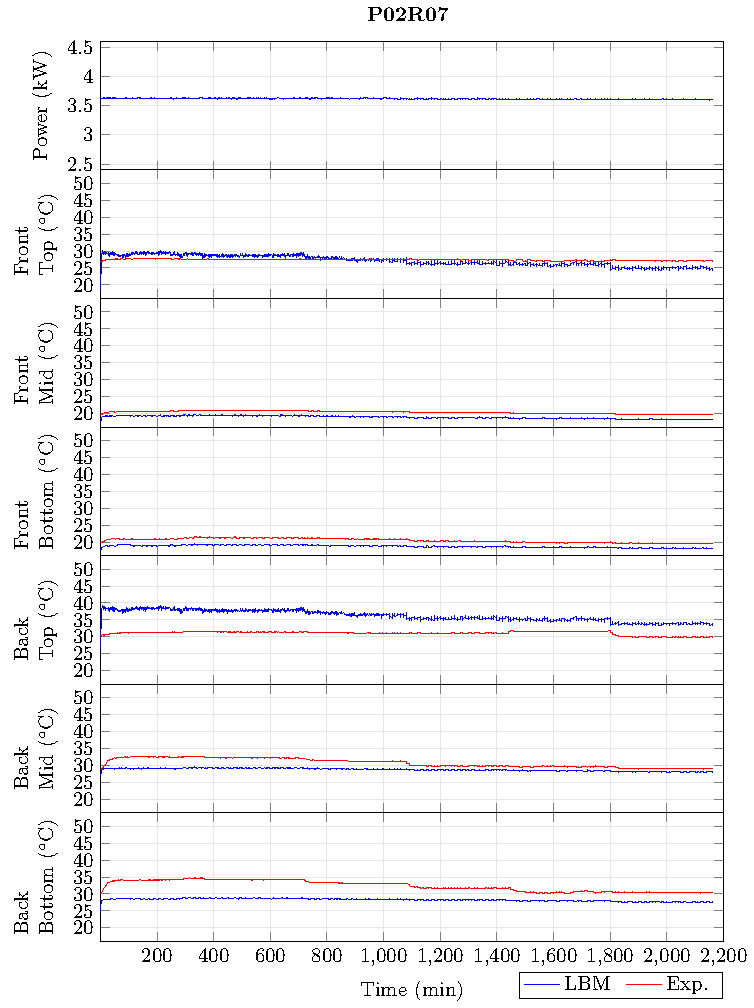
\includegraphics[width=\linewidth]{Plots/P02R07_T.pdf}
\caption{Comparison of simulated and experimental temperatures for server P02R07.}
\label{fig:P02R07_plot}
\end{figure}

\clearpage

% P02R08
\begin{figure}[!htb]
\centering
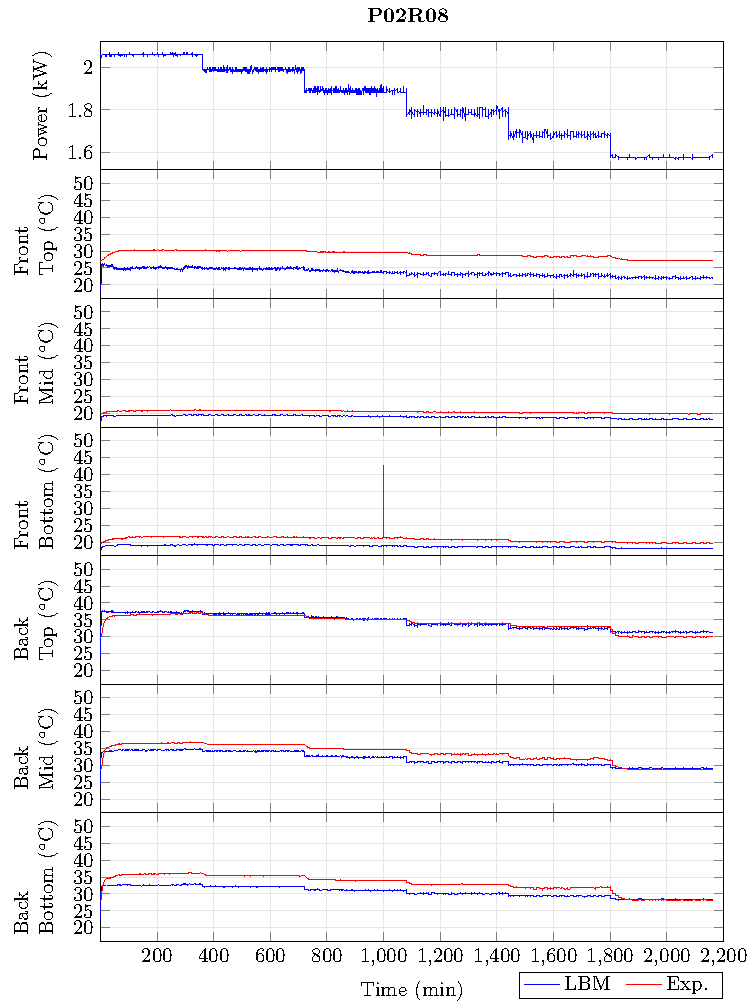
\includegraphics[width=\linewidth]{Plots/P02R08_T.pdf}
\caption{Comparison of simulated and experimental temperatures for server P02R08.}
\label{fig:P02R08_plot}
\end{figure}

\clearpage

% P02R09
\begin{figure}[!htb]
\centering
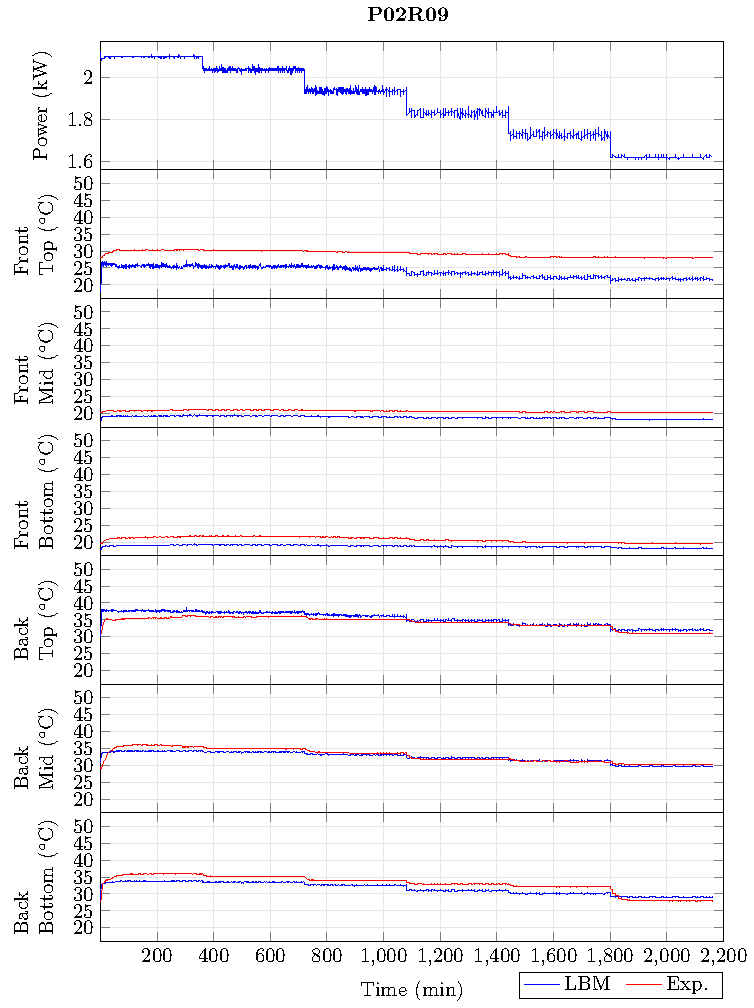
\includegraphics[width=\linewidth]{Plots/P02R09_T.pdf}
\caption{Comparison of simulated and experimental temperatures for server P02R09.}
\label{fig:P02R09_plot}
\end{figure}

\clearpage

% P02R10
\begin{figure}[!htb]
\centering
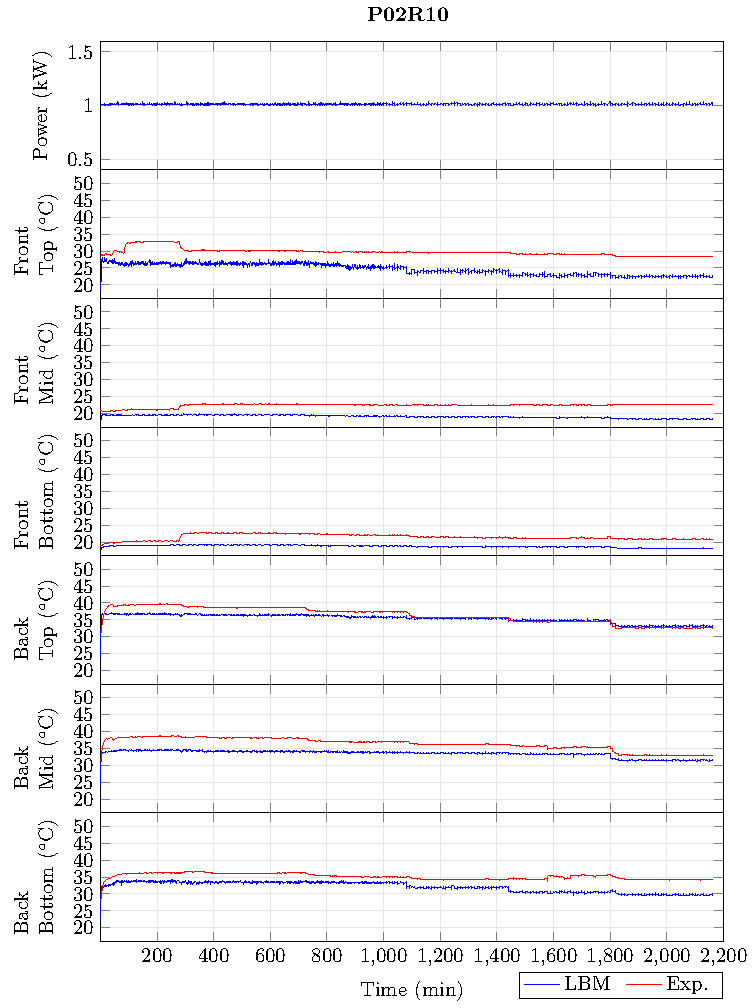
\includegraphics[width=\linewidth]{Plots/P02R10_T.pdf}
\caption{Comparison of simulated and experimental temperatures for server P02R10.}
\label{fig:P02R10_plot}
\end{figure}

\end{document}
